\scanpage{30}

% L1–2 upper left
\[
 \begin{matrix}\unsure{\zeta|\xi}_1&\zeta_2&\zeta_3&\zeta_{32}\\
 \zeta'_1&\zeta'_2&\zeta'_3&\end{matrix}
\]

% L1 upper centre
\figure{\begin{tikzpicture}\draw[|-|] (0,0)--(1.65,0);\draw[|-|] (1.7,0)--(3.4,0);\end{tikzpicture}}

% L1 upper right
\[
 \frac{72\cdot6!=72\cdot720}{72\cdot6}=120
\]

% L3–4 left
\diagram{\begin{tikzcd}[ampersand replacement=\&,column sep=small]
 \zeta_1\zeta_2\zeta_3 \& \zeta_4\zeta_5\zeta_6\arrow[r,dash]\& \underline{\zeta_{12}\zeta_{23}\zeta_{34}}\\
 \zeta'_1\zeta'_2\zeta'_3 \& \zeta'_4\deleted{\unsure{*}}\zeta'_5\zeta'_6\arrow[ur,dash]\&\zeta_{45}\zeta_{56}\zeta_{6\unsure{1|4}}
\end{tikzcd}}

% L2–8 upper right
\diagram{\begin{tikzcd}[ampersand replacement=\&,row sep=1ex,column sep=1em,execute at end picture={\draw ([xshift=2pt]current bounding box.north east)--([xshift=-3pt,yshift=-3pt]current bounding box.north west)--([xshift=-3pt,yshift=3pt]current bounding box.south west)--(current bounding box.south east);} ]
 \text{trièdres}\arrow[r,leftrightarrow]\&\text{hexagones}\\
 \text{hex. trièdres}\arrow[r,leftrightarrow]\arrow[d,leftrightarrow]\&\text{bitriangles}\arrow[d,leftrightarrow]\\
 \text{plan } A_2\arrow[r,leftrightarrow]\&\text{bloc de trièdres}\\
 \text{trihexatrièdres}\arrow[r,leftrightarrow]\arrow[d,leftrightarrow]\& \deleted{\unsure{\text{trièdres}}}\,\text{\unsure{triplets|triples de} bitriangles}\arrow[d,leftrightarrow]\\
 \text{décomposition}\arrow[r,dash]\arrow[d,leftrightarrow]\&\text{\unsure{triplet|triple} \unsure{tribloc|bloc} de trièdres}\\
 \deleted{\unsure{\text{triple }A_2|A_2\,\ldots\,A_2}}\ \text{triplan } A_2 \&
\end{tikzcd}}

% centre left
\diagram{\begin{tikzcd}[ampersand replacement=\&,row sep=2ex,column sep=1em]
 \&\underline{\zeta_{12}\zeta_{23}\zeta_{34}}\arrow[dl,dash,"-r_6"']\arrow[dr,dash,"r_{456}"]\&\\
 \zeta'_4\zeta'_5\zeta'_6\arrow[d,dash,"{-r_{\deleted{\unsure{6}}0}} "']\&\&\zeta_4\zeta_5\zeta_6\arrow[d,dash,"r_0"]\\
 \zeta'_1\zeta'_2\zeta'_3\arrow[dr,dash,"-r_{456}"']\&\&\zeta_1\overline{\zeta_2}\zeta_3\arrow[dl,dash,"r_6"]\\
 \&\underline{\zeta_{45}\zeta_{56}\zeta_{61}}\&
\end{tikzcd}}

% centre right
\[
 \zeta_{ij}\quad\begin{matrix}1\le i\le3\\4\le j\le6\end{matrix}
 \qquad
 \begin{matrix}\zeta_{14}&\zeta_{15}&\zeta_{16}\\\zeta_{24}&\zeta_{25}&\zeta_{\underline{26}}\\\zeta_{34}&\zeta_{35}&\zeta_{36}\end{matrix}
\]

% centre below hexagon
\figure{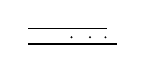
\begin{tikzpicture}[scale=.5]\draw (0,.4)--(2,.4) (0,0)--(2.25,0);\foreach \x in {1.1,1.57,1.96}{\fill (\x,.17) circle (.8pt);}\end{tikzpicture}}

% L10–12
NB de 3 bases (\unsure{ou couples|un couple} de racines : $60^\circ$)

% L11–13
\[
 36\cdot\underbrace{\binom63\deleted{\unsure{2/2|4/24}}}_{\frac{6\cdot5\cdot4}{3!\,\unsure{2^2|2!}}=20}=720
 \qquad\begin{aligned}&\text{nb de paires de}\\&\text{racines faisant }60^\circ\end{aligned}
\]

% L14
plan $A_2$ : $\dfrac{720}{6}=120$ \(\mathbin{/\mkern-4mu/}\)

% lower right
\[
 \begin{matrix}
 \zeta_{14}&\zeta_{25}&\zeta_{36}\\
 \zeta_{26}&\zeta_{34}&\zeta_{15}\\
 \zeta_{35}&\zeta_{16}&\zeta_{24}
 \end{matrix}
\]

% lower left
\diagram{\begin{tikzcd}[ampersand replacement=\&,row sep=1ex,column sep=small]
 \deleted{\text{plan }A_2}\&\\
 \text{sous syst. }A_2\arrow[d,leftrightarrow]\&\\
 \text{\unsure{3bloc|3 blocs} de \unsure{3trièdres|bitriades}}\arrow[d,leftrightarrow]\&
 \unsure{\mathfrak S|\mathfrak G}_2\cdot(\mathfrak S_3\times\mathfrak S_3)\\
 \text{bitriangle}\arrow[d,leftrightarrow]\arrow[ur,phantom,"\smash{\raisebox{.7ex}{$\left.\rule{0pt}{4.3ex}\right\}$}}" description]\& \mathfrak S_3\cdot(\mathfrak S_3\times\mathfrak S_3\times\mathfrak S_3)\\
 \text{hexagone de trièdres.}\&
\end{tikzcd}}

% foot right
\[
 \begin{matrix}
 \bullet\\[-2pt]\triangle\\[-2pt]\cdot\ \cdot\ \cdot\ \cdot\ \cdot\ \cdot\\[-2pt]
 \deleted{\unsure{\boxplus}}\ \text{\unsure{tribloc|triple}}
 \end{matrix}
 \quad
 \left\{\begin{array}{lr}
 \text{sommets}&27\\\text{triangles}&45\\\text{bibase}&36\\\text{trois-neufs}&40
 \end{array}\right.
\]
% archive sheet number: 29
